\documentclass[tikz,convert=false]{standalone}
\usetikzlibrary{automata}
\usetikzlibrary{positioning}
\begin{document}
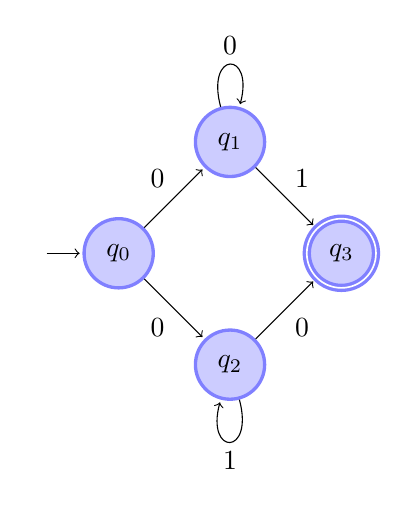
\begin{tikzpicture}[shorten >=1pt,node distance=2cm,on grid,%
  initial text=,every state/.style={draw=blue!50,%
  very thick,fill=blue!20}]
  \node[state,initial]   (q0)                       {$q_{0}$};
  \node[state]           (q1) [above right = of q0] {$q_{1}$};
  \node[state]           (q2) [below right = of q0] {$q_{2}$};
  \node[state,accepting] (q3) [below right = of q1] {$q_{3}$};

  \path[->] (q0) edge              node [above left]  {0} (q1)
                 edge              node [below left]  {0} (q2)
            (q1) edge              node [above right] {1} (q3)
                 edge [loop above] node               {0} ()
            (q2) edge              node [below right] {0} (q3)
                 edge [loop below] node               {1} ();
\end{tikzpicture}
\end{document}
